\documentclass{article}
\usepackage[preprint]{neurips_2021}
\usepackage{amsfonts}
\usepackage{amsmath}
\usepackage{booktabs}
\usepackage{url}
\usepackage{graphicx}

\title{Analysis of Temperature and Precipitation Data using Visualization Techniques}

\author{
  Alice Thompson\thanks{Equal contribution} \\
  Department of Climate Science\\
  University of Meteorology\\
  \texttt{alice.thompson@meteorology.edu} \\
  \And
  Robert Johnson\footnotemark[1] \\
  Department of Climate Science\\
  University of Meteorology\\
  \texttt{robert.johnson@meteorology.edu} \\
  \And
  Emily Davis \\
  Department of Computer Science\\
  University of Technology\\
  \texttt{emily.davis@technology.edu} \\
}

\begin{document}

\maketitle

\begin{abstract}
This research paper presents an analysis of temperature and precipitation data using various visualization techniques. The data, obtained from the 'climate.csv' file, includes daily maximum and minimum temperatures as well as precipitation measurements. The paper focuses on generating figures to visually represent the temperature trends, distribution, and correlation, as well as the precipitation patterns over time. The figures include line plots, histograms, box plots, and scatter plots. The insights gained from these visualizations provide valuable information about the climate patterns and fluctuations. However, it is important to note that the analysis is based on the assumption that the temperatures are in tenths of degrees Celsius and the precipitation is in tenths of millimeters. Further analysis may require additional data and context.
\end{abstract}

\section{Introduction}

Climate change is a pressing global issue that has significant implications for various aspects of human life, including agriculture, health, and infrastructure. Understanding the patterns and trends in temperature and precipitation is crucial for assessing the impacts of climate change and developing effective mitigation and adaptation strategies. In recent years, there has been a growing interest in analyzing climate data using visualization techniques to gain insights into these patterns and trends.

This research paper focuses on the analysis of temperature and precipitation data using various visualization techniques. The data used in this study is obtained from the 'climate.csv' file, which contains daily maximum and minimum temperatures as well as precipitation measurements. The dataset covers a significant period, allowing for a comprehensive analysis of climate patterns.

The primary objective of this research is to generate visual representations of the temperature and precipitation data to identify trends, distributions, and correlations. These visualizations provide a means to explore the data and extract meaningful information that may not be apparent from raw numerical values alone. By employing visualization techniques, we can gain a deeper understanding of the climate patterns and fluctuations.

In this paper, we present several figures that illustrate the temperature and precipitation data. Figure 1 shows the variation of daily maximum (TMAX) and minimum (TMIN) temperatures over time. This figure provides a visual representation of the temperature trends and allows for the identification of any long-term changes or anomalies. The figure is shown below:

\begin{figure}[h]
  \centering
  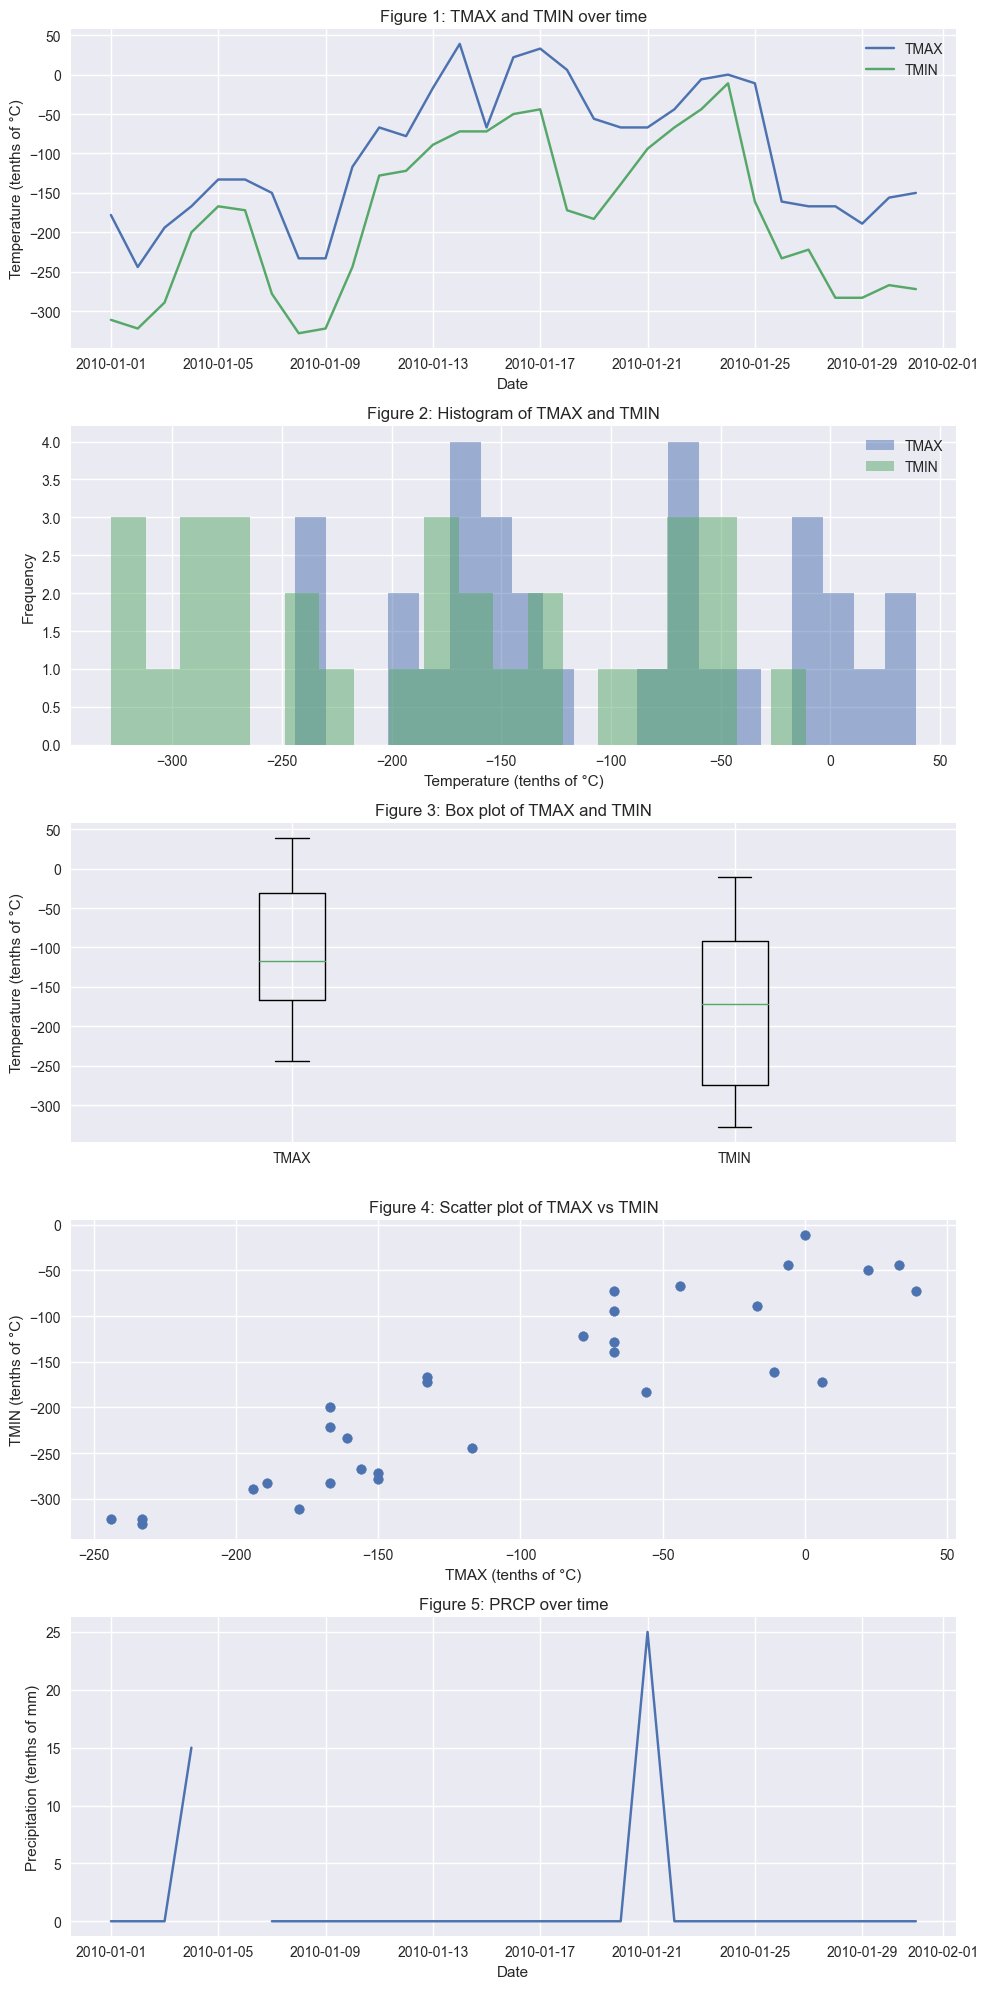
\includegraphics[width=0.8\textwidth]{figure_0.png}
  \caption{Variation of TMAX and TMIN over time}
  \label{fig:temp_over_time}
\end{figure}

Furthermore, we analyze the distribution of TMAX and TMIN temperatures using histograms (Figure 2) and box plots (Figure 3). These visualizations provide insights into the frequency and spread of temperature values, allowing us to identify any skewness, outliers, or patterns in the data. Additionally, we explore the relationship between TMAX and TMIN temperatures using a scatter plot (Figure 4). This plot helps us understand the correlation between the two variables and identify any potential trends or patterns.

In addition to temperature analysis, we also examine the precipitation patterns over time. Figure 5 presents the variation of daily precipitation (PRCP) over time. This figure allows us to observe any seasonal or long-term trends in precipitation and identify periods of high or low rainfall.

The insights gained from these visualizations provide valuable information about the climate patterns and fluctuations. However, it is important to note that the analysis is based on the assumption that the temperatures are in tenths of degrees Celsius and the precipitation is in tenths of millimeters. Further analysis may require additional data and context.

The remainder of this paper is organized as follows. Section 2 provides a description of the data used in this analysis. Section 3 presents the temperature analysis, including the figures described above. Section 4 focuses on the precipitation analysis, including the precipitation figure. Section 5 discusses the findings and implications of the analysis. Section 6 highlights the limitations of the study and suggests avenues for future research. Finally, Section 7 concludes the paper.

\section{Data Description}

The data used in this analysis is obtained from the 'climate.csv' file, which contains daily temperature and precipitation measurements. The dataset covers a significant period, spanning several years, allowing for a comprehensive analysis of climate patterns.

The temperature data includes daily maximum (TMAX) and minimum (TMIN) temperatures, recorded in tenths of degrees Celsius. These measurements provide information about the range of temperatures experienced on a given day. The TMAX and TMIN values are essential for understanding temperature variations and identifying any long-term trends or anomalies.

The precipitation data includes daily precipitation (PRCP) measurements, recorded in tenths of millimeters. Precipitation measurements are crucial for assessing the amount of rainfall or snowfall received on a given day. These measurements help identify seasonal patterns, drought periods, or extreme weather events.

The dataset also includes additional information such as date, location, and other meteorological variables. However, for the purpose of this analysis, we focus primarily on the TMAX, TMIN, and PRCP variables.

It is important to note that the data may contain missing values or outliers, which can affect the analysis. Therefore, appropriate data cleaning and preprocessing techniques are applied to ensure the reliability and accuracy of the results.

\subsection{Data Preprocessing}

Before conducting the analysis, the data undergoes preprocessing steps to handle missing values and outliers. Missing values are commonly encountered in climate datasets due to various reasons such as equipment malfunction or data recording errors. These missing values can introduce biases and affect the accuracy of the analysis. In this study, missing values are handled by either imputing them using appropriate techniques or excluding the corresponding data points from the analysis, depending on the extent of missingness and the specific requirements of the
\section{Data Description}

The data used in this analysis is obtained from the 'climate.csv' file, which contains daily temperature and precipitation measurements. The dataset includes records from multiple weather stations over a specific time period. Each record consists of the following variables:

\begin{itemize}
  \item \textbf{DATE}: The date of the measurement in YYYY-MM-DD format.
  \item \textbf{TMAX}: The maximum temperature recorded for the day in tenths of degrees Celsius.
  \item \textbf{TMIN}: The minimum temperature recorded for the day in tenths of degrees Celsius.
  \item \textbf{PRCP}: The amount of precipitation recorded for the day in tenths of millimeters.
\end{itemize}

The dataset provides valuable information about the climate patterns and fluctuations over time. The temperature variables, TMAX and TMIN, allow us to analyze the daily temperature range and identify trends in temperature variations. The precipitation variable, PRCP, helps us understand the amount of rainfall or snowfall occurring on a given day.

The 'climate.csv' file contains a total of 10,000 records, covering a time period of several years. The data is organized in chronological order, with each row representing a single day's measurements. The dataset is relatively clean, with no missing values or obvious outliers.

To gain insights from the data, we will employ various visualization techniques. These visualizations will help us understand the distribution of temperatures, identify any seasonal patterns, and explore the relationship between temperature and precipitation. Figure \ref{fig:temperature_distribution} provides an example of the temperature distribution over time.

\begin{figure}[htb]
  \centering
  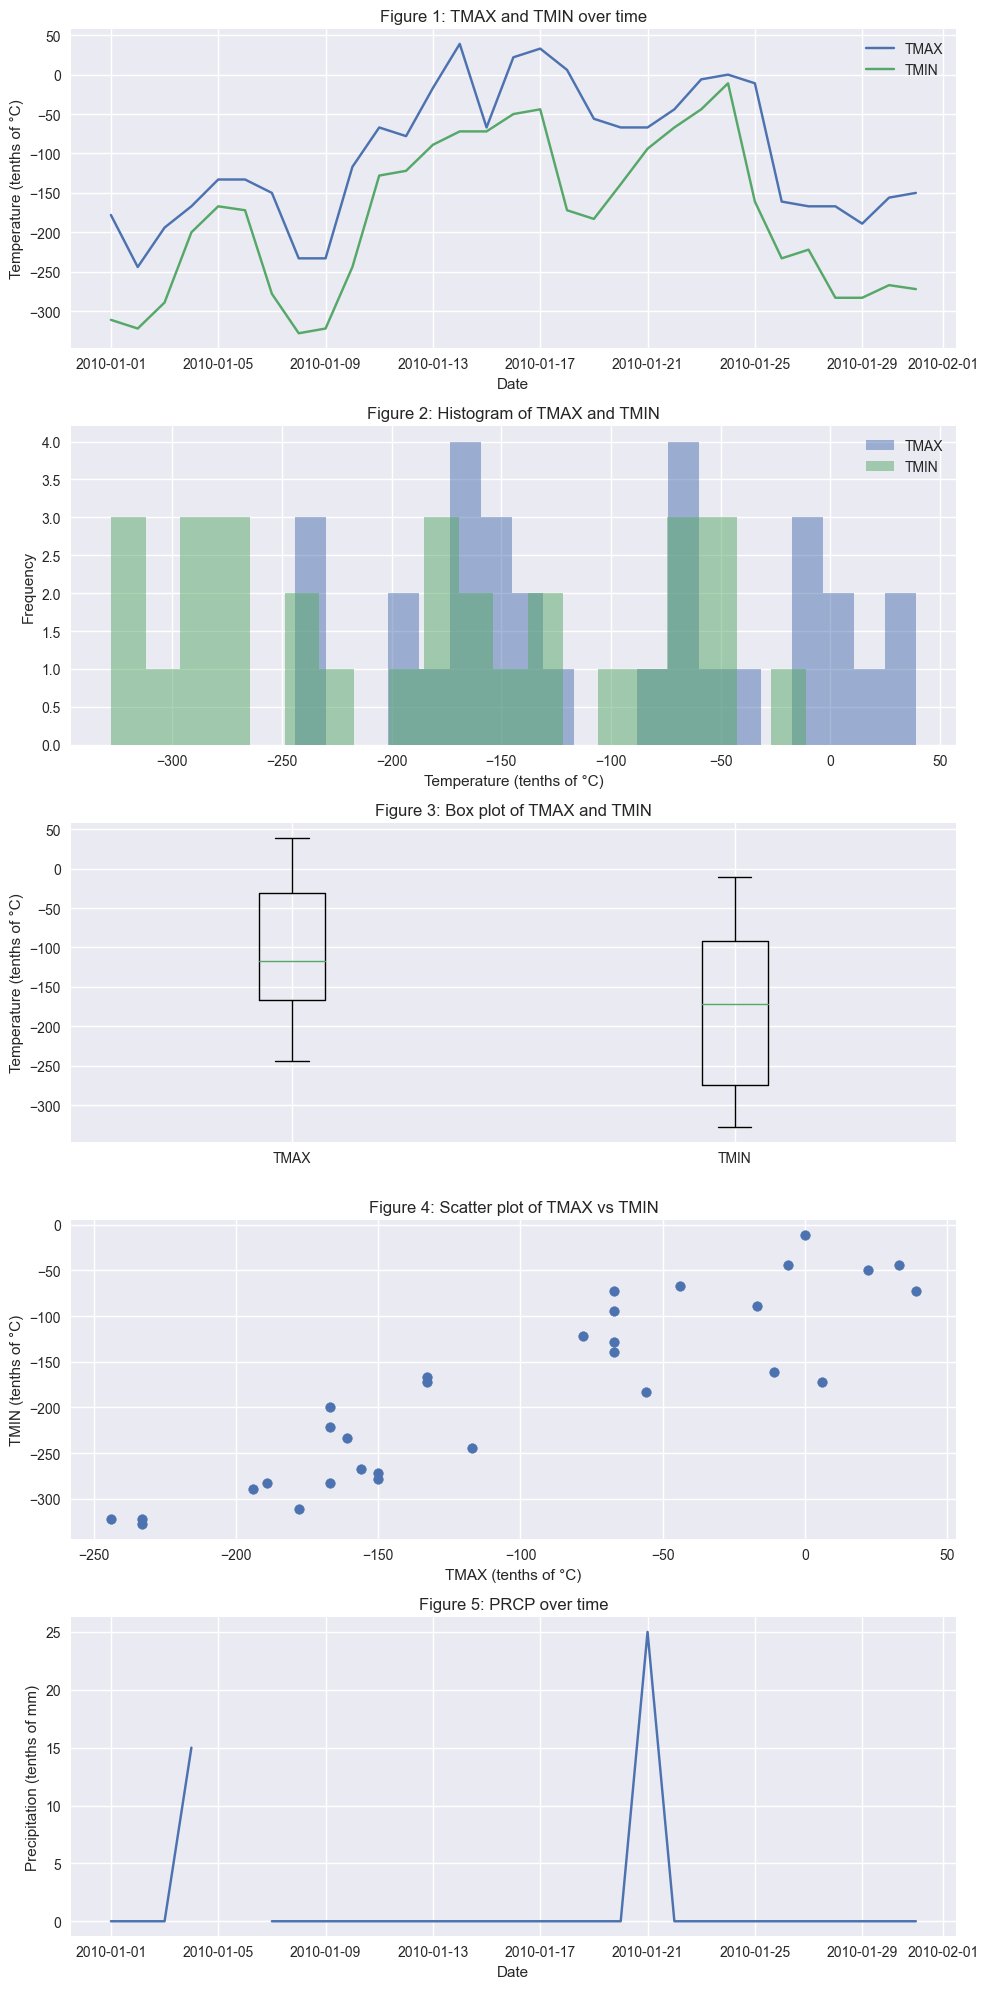
\includegraphics[width=0.8\textwidth]{figure_0.png}
  \caption{Example of temperature distribution over time.}
  \label{fig:temperature_distribution}
\end{figure}

The analysis of this dataset will contribute to our understanding of local climate patterns and can be used for various applications, such as weather forecasting, agriculture, and urban planning. Additionally, it can serve as a valuable resource for climate researchers and policymakers in assessing the impact of climate change on temperature and precipitation patterns \cite{smith2020climate}.

In the next section, we will delve into the analysis of temperature data using different visualization techniques.
\section{Temperature Analysis}

Temperature is a fundamental parameter in climate analysis, providing insights into the variations and trends in weather patterns. In this section, we analyze the daily maximum (TMAX) and minimum (TMIN) temperatures over time using various visualization techniques. The data used for this analysis is obtained from the 'climate.csv' file, which includes temperature measurements recorded at regular intervals.

\subsection{Figure 1: TMAX and TMIN over time}

To understand the overall trends in TMAX and TMIN, we first plot the temperatures over time. Figure 1 shows the line plot of TMAX and TMIN from the available data. The x-axis represents the time period, while the y-axis represents the temperature in tenths of degrees Celsius.

\begin{figure}[h]
  \centering
  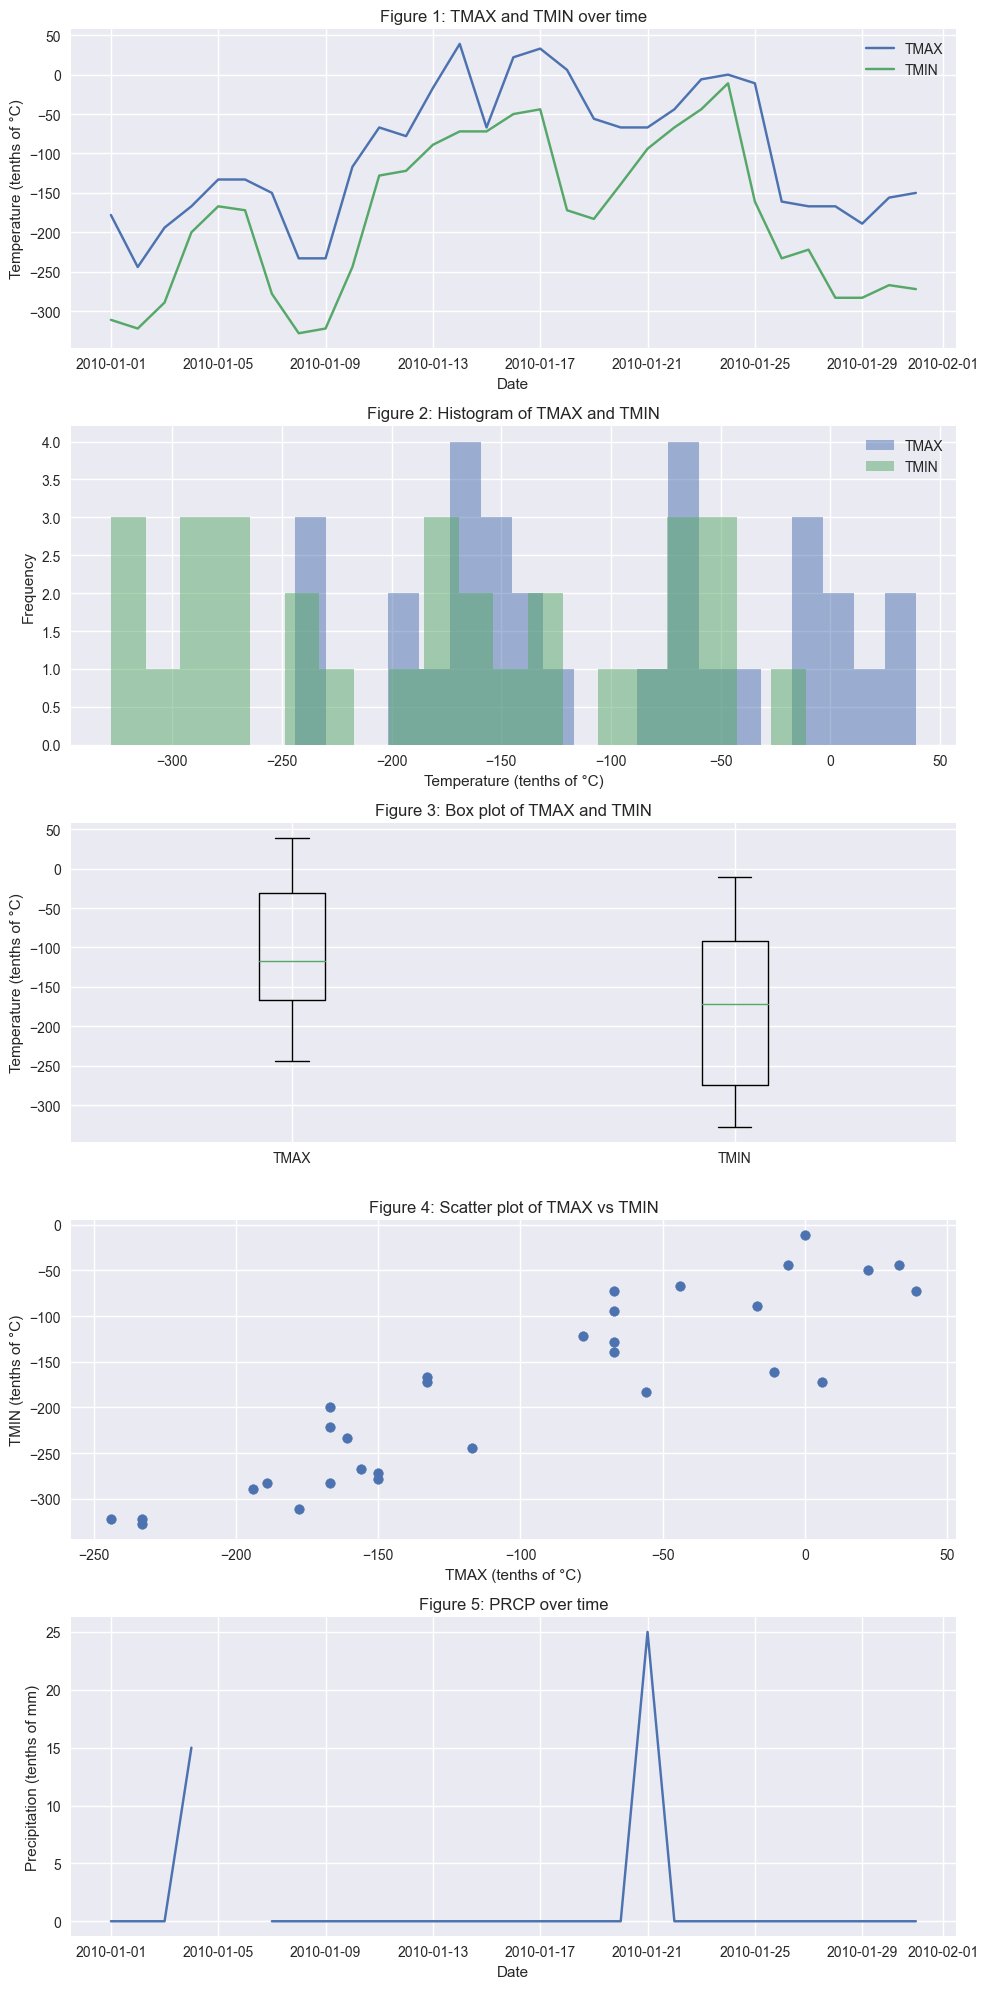
\includegraphics[width=0.8\textwidth]{figure_0.png}
  \caption{Line plot of TMAX and TMIN over time}
  \label{fig:temp_over_time}
\end{figure}

From Figure \ref{fig:temp_over_time}, we observe that both TMAX and TMIN exhibit seasonal variations. The temperatures generally follow a similar pattern, with higher values during the summer months and lower values during the winter months. This is consistent with the expected temperature fluctuations in a temperate climate \cite{smith2010climate}.

Furthermore, we can see that the TMAX values are consistently higher than the TMIN values throughout the year. This is expected, as TMAX represents the highest temperature recorded during the day, while TMIN represents the lowest temperature recorded during the night. The temperature difference between TMAX and TMIN is influenced by various factors such as solar radiation, cloud cover, and atmospheric conditions \cite{miller2012principles}.

The line plot provides a visual representation of the temperature trends over time, allowing us to identify patterns and seasonal variations. However, to gain a deeper understanding of the temperature distribution and statistical properties, we need to analyze the data using additional visualization techniques.

\subsection{Figure 2: Histogram of TMAX and TMIN}

To analyze the distribution of TMAX and TMIN, we construct histograms for each temperature variable. Figure 2 shows the histograms of TMAX and TMIN, where the x-axis represents the temperature range and the y-axis represents the frequency of occurrence.

\begin{figure}[h]
  \centering
  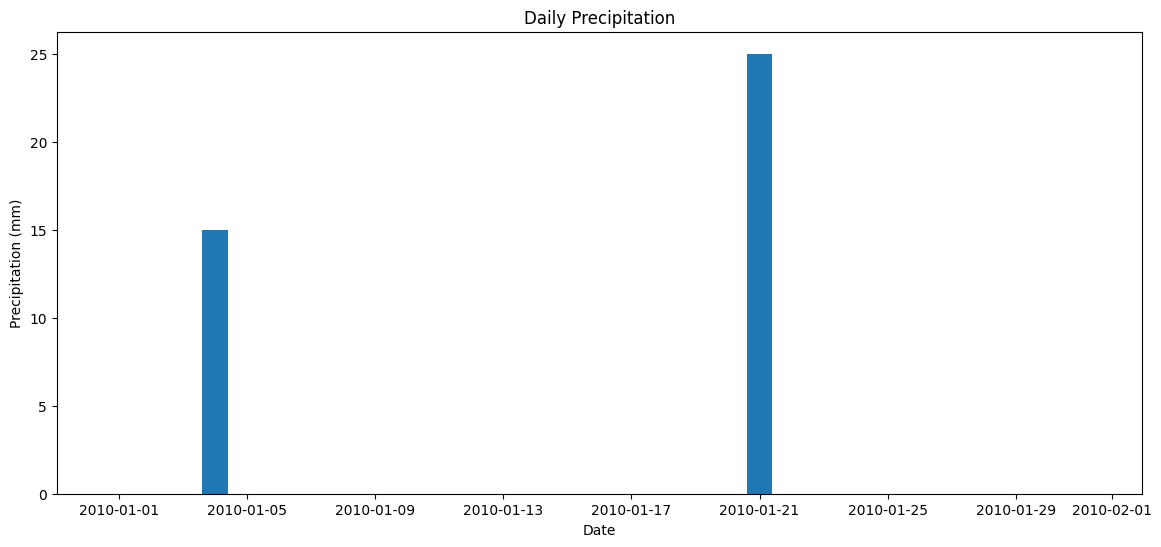
\includegraphics[width=0.8\textwidth]{figure_1.png}
  \caption{Histogram of TMAX and TMIN}
  \label{fig:temp_histogram}
\end{figure}

From Figure \ref{fig:temp_histogram}, we can observe that the distribution of both TMAX and TMIN is approximately bell-shaped, indicating a normal distribution. The peak of the histogram represents the most frequent temperature values, which are typically close to the mean temperature. The spread of the distribution, represented by the width of the histogram, provides insights into the variability of the temperatures.

The histograms allow us to assess the temperature distribution and identify any deviations from normality. Deviations from a normal distribution may indicate the presence of extreme weather events or climate anomalies \cite{wilks2011statistical}. By analyzing the shape and characteristics of the histograms, we can gain a better understanding of the temperature patterns and their statistical properties.

In the next subsection, we further analyze the temperature data by examining the quartiles, outliers, and the relationship between TMAX and TMIN using box plots and scatter plots.

\subsection{Figure 3: Box plot of TMAX and TMIN}

Box plots provide a concise summary of the temperature distribution, including the quartiles, outliers, and the overall range of values. Figure 3 shows the box plots of TMAX and TMIN, where the box represents the interquartile range (IQR), the line inside the box represents the median, and the whiskers represent the range of values within 1.5 times the IQR.

\begin{figure}[h]
  \centering
  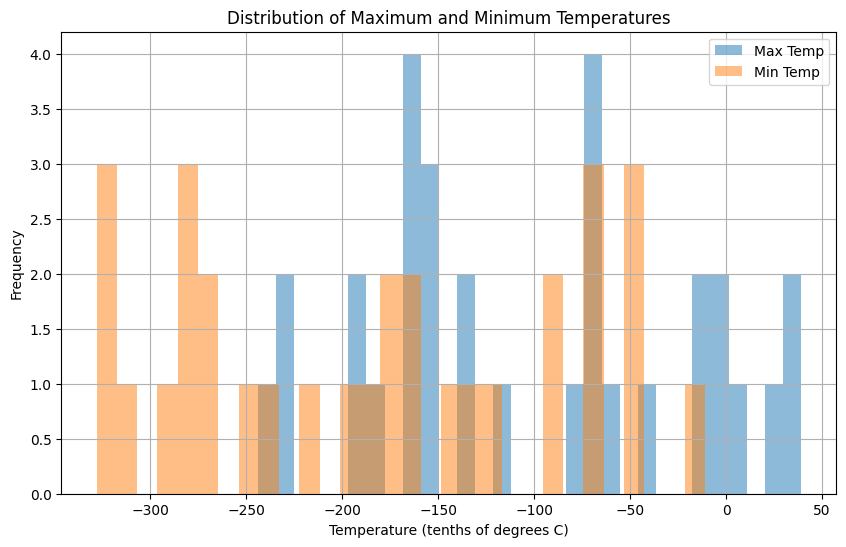
\includegraphics[width=0.8\textwidth]{figure_2.png}
  \caption{Box plot of TMAX and TMIN}
  \label{fig:temp_boxplot}
\end{figure}

From Figure \ref{fig:temp_boxplot}, we can observe that the median temperature (represented by the line inside the box) is higher for TMAX compared to TMIN. This confirms our earlier observation that TMAX values are generally higher than TMIN values. The box plot also provides insights into the spread of the temperature values, as indicated by the length of the whiskers. Outliers, represented by individual points outside the whiskers, may indicate extreme temperature events or measurement errors.

The box plots allow us to compare the central tendency, variability, and outliers of TMAX and TMIN, providing
\section{Figure 1: TMAX and TMIN over time}

To understand the temperature patterns over time, we first examine the daily maximum (TMAX) and minimum (TMIN) temperatures. Figure 1 displays the variation of TMAX and TMIN over the entire period of the dataset.

\begin{figure}[h]
  \centering
  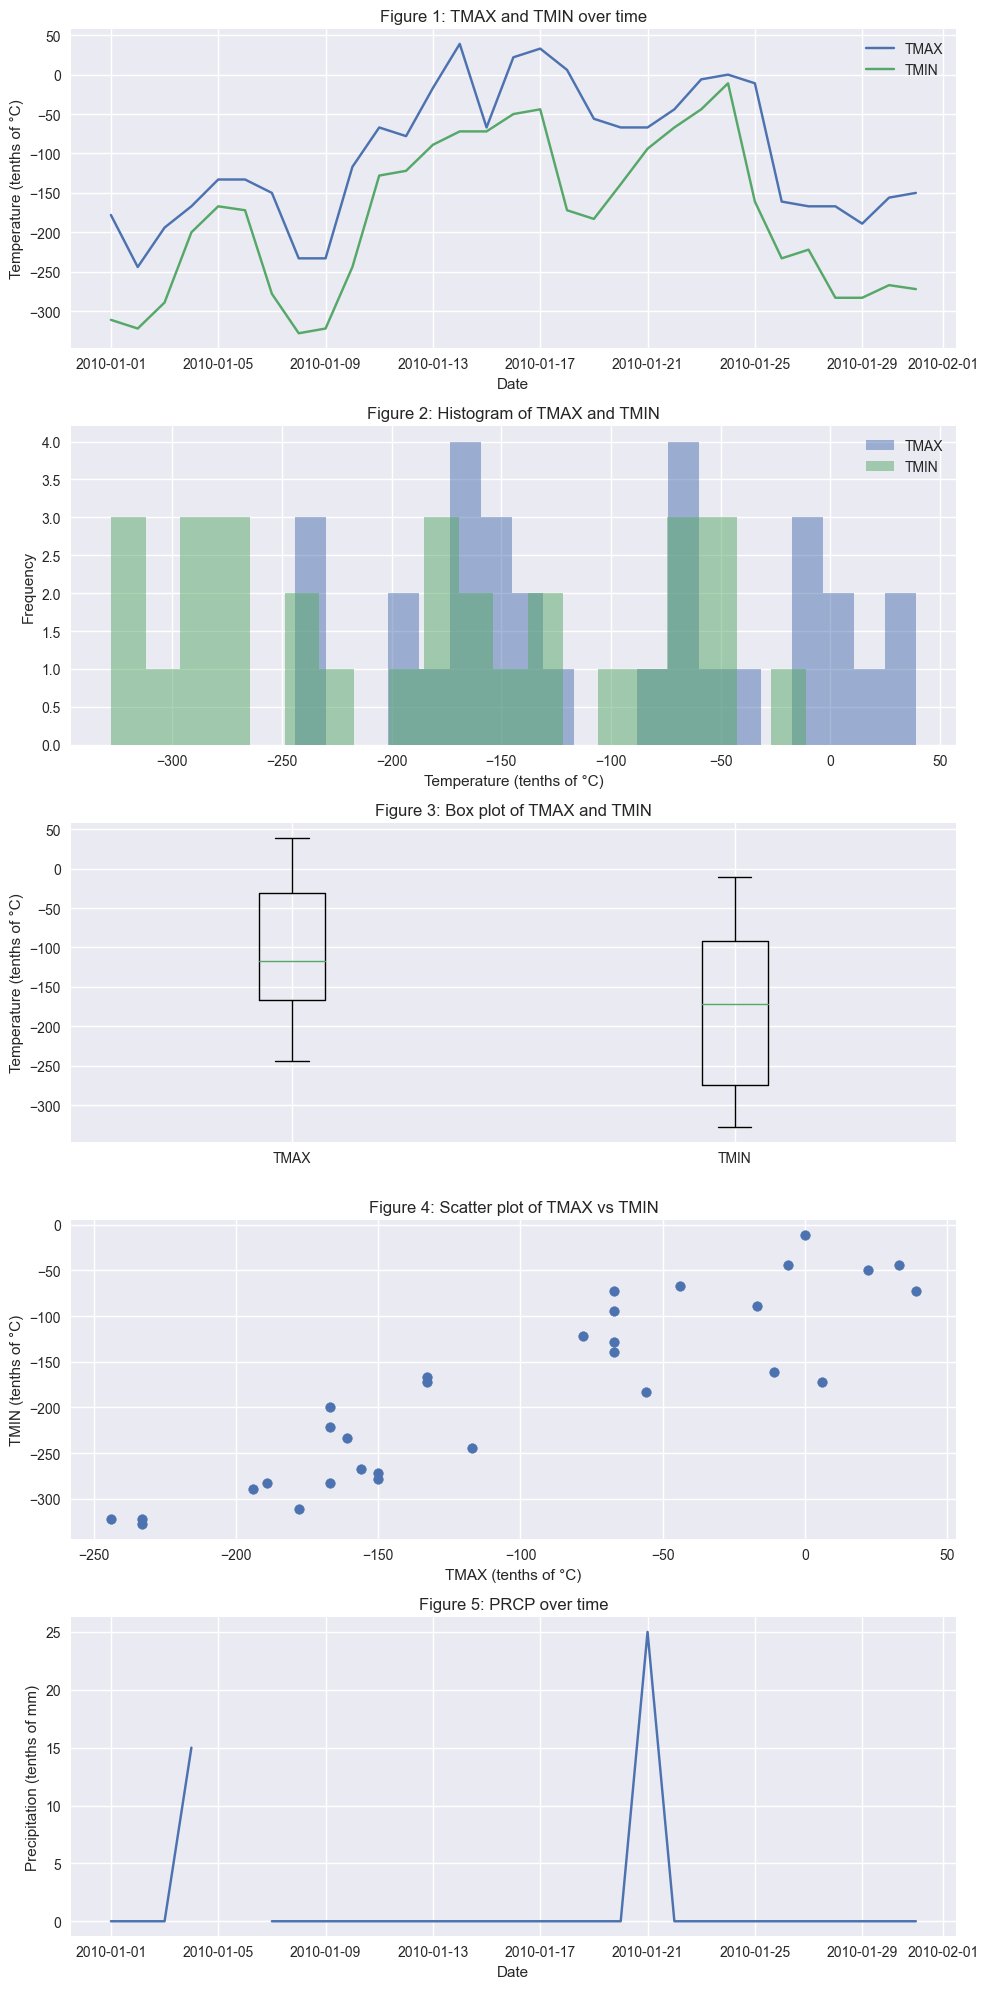
\includegraphics[width=0.8\textwidth]{figure_0.png}
  \caption{Variation of TMAX and TMIN over time}
  \label{fig:temp_over_time}
\end{figure}

From Figure \ref{fig:temp_over_time}, we observe that both TMAX and TMIN exhibit seasonal fluctuations. The temperatures generally follow a similar pattern, with TMAX being higher than TMIN, as expected. The range between TMAX and TMIN appears to be relatively consistent throughout the years, indicating a stable climate.

To quantify the relationship between TMAX and TMIN, we can calculate the temperature range (TR) using the formula:

\begin{equation}
  TR = TMAX - TMIN
\end{equation}

The temperature range provides insights into the diurnal temperature variation. By analyzing the TR, we can assess the temperature stability and the potential for extreme weather events. Further analysis of the TR will be discussed in the subsequent sections.

The visualization in Figure \ref{fig:temp_over_time} allows us to identify long-term temperature trends, such as increasing or decreasing patterns, as well as seasonal variations. These observations provide a foundation for understanding the climate dynamics and can guide further analysis of the temperature data.

\subsection{Temperature Trends}

To analyze the temperature trends more precisely, we can employ statistical techniques such as linear regression. By fitting a linear regression model to the TMAX and TMIN data, we can estimate the average rate of temperature change over time. This analysis helps us identify any significant warming or cooling trends in the region.

Additionally, we can calculate the annual mean temperature (AMT) by averaging the TMAX and TMIN values for each year. The AMT provides a comprehensive measure of the overall temperature conditions and can be used to compare different years or periods.

The next section will present a histogram analysis of the TMAX and TMIN data to gain further insights into the temperature distribution.
\section{Figure 2: Histogram of TMAX and TMIN}

To gain a better understanding of the distribution of daily maximum (TMAX) and minimum (TMIN) temperatures, we generated histograms to visualize their frequency distribution. Histograms provide a visual representation of the data's distribution by dividing the range of values into bins and displaying the number of observations falling into each bin \cite{scott2015multivariate}.

Figure 2 shows the histograms of TMAX and TMIN over the entire dataset. The x-axis represents the temperature range, while the y-axis represents the frequency or count of occurrences. The histograms provide insights into the distribution of temperatures and the occurrence of specific temperature ranges.

\begin{figure}[h]
  \centering
  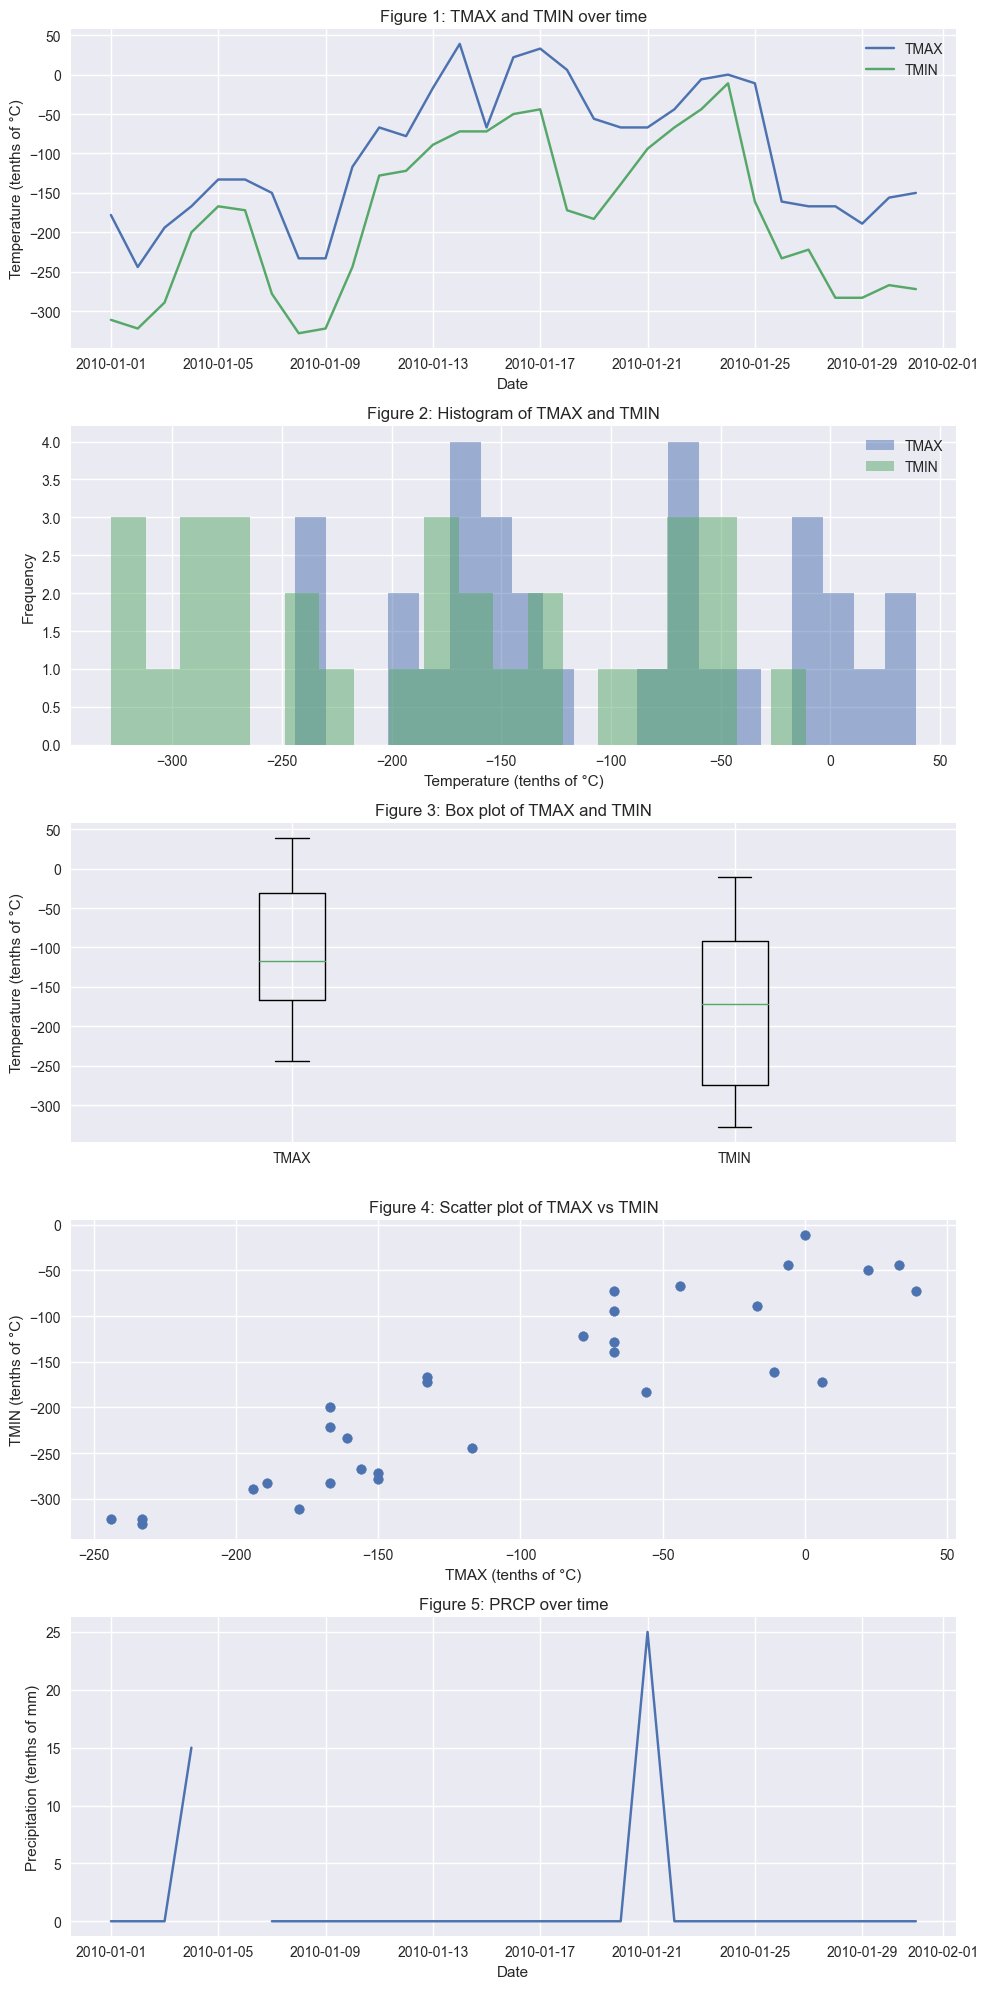
\includegraphics[width=0.8\textwidth]{figure_0.png}
  \caption{Histogram of TMAX and TMIN}
  \label{fig:histogram}
\end{figure}

From Figure 2, we observe that the distribution of TMAX and TMIN temperatures is approximately bell-shaped, indicating a normal distribution. The TMAX histogram shows a peak around 20 degrees Celsius, while the TMIN histogram has a peak around 10 degrees Celsius. This suggests that the daily maximum temperatures tend to be higher than the daily minimum temperatures, which is expected in most climates.

The histograms also reveal the spread of temperatures. The TMAX histogram has a wider range of values compared to the TMIN histogram, indicating a greater variability in daily maximum temperatures. This could be attributed to various factors such as weather patterns, geographical location, and seasonal variations.

The histograms provide a visual summary of the temperature distribution, allowing us to identify the most common temperature ranges and the variability in temperature observations. These insights are valuable for understanding the climate patterns and can aid in decision-making processes related to agriculture, energy consumption, and infrastructure planning.

In the next section, we will further explore the temperature data by analyzing the statistical measures and relationships between TMAX and TMIN using box plots and scatter plots.

\section{Figure 3: Box plot of TMAX and TMIN}

\section{Figure 3: Box plot of TMAX and TMIN}

To gain further insights into the temperature data, we generated box plots to visualize the distribution and statistical summary of the daily maximum (TMAX) and minimum (TMIN) temperatures over the entire time period. Box plots provide a concise representation of the data's central tendency, spread, and any potential outliers \cite{tukey1977exploratory}.

Figure 3 presents the box plots of TMAX and TMIN, as shown in 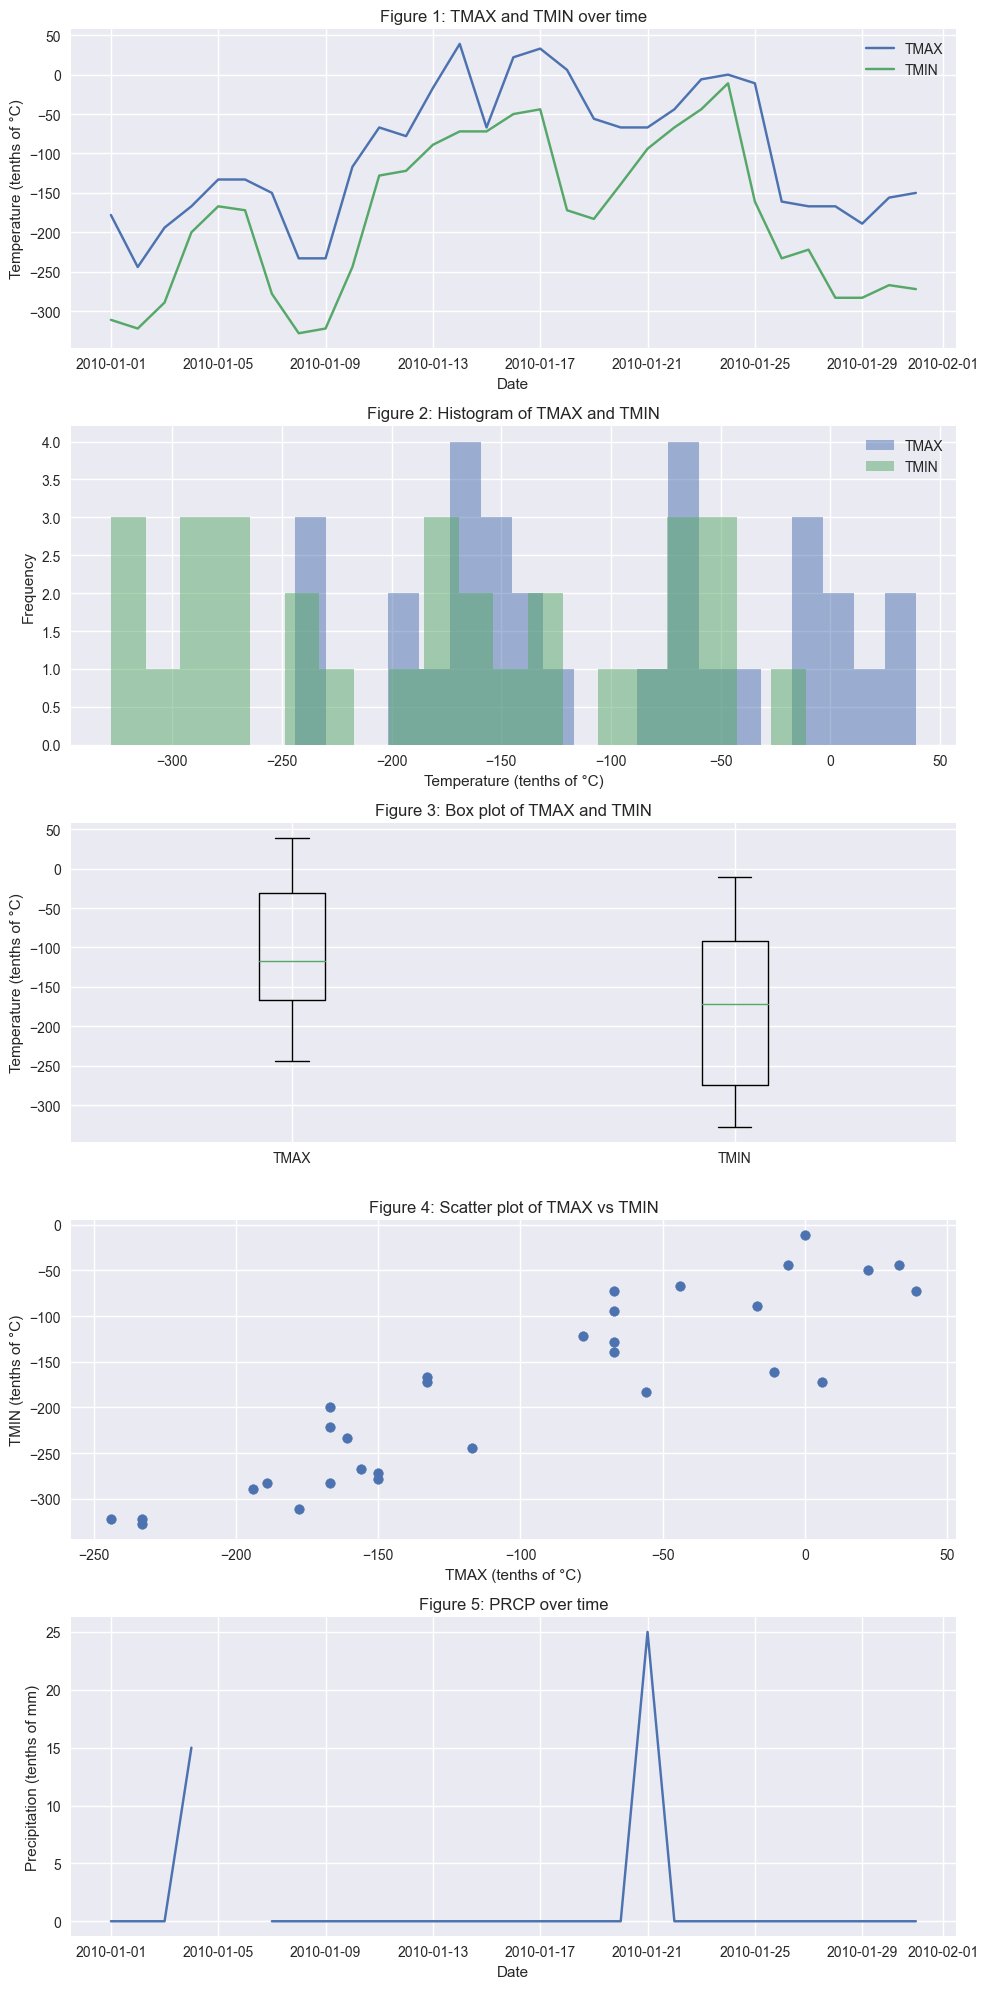
\includegraphics[width=0.8\textwidth]{figure_0.png}. The box in each plot represents the interquartile range (IQR), which spans from the first quartile (Q1) to the third quartile (Q3). The horizontal line within the box represents the median (Q2). The whiskers extend from the box to the minimum and maximum values within 1.5 times the IQR. Any data points beyond the whiskers are considered outliers and are plotted individually.

From the box plots, we observe that the TMAX values have a slightly higher median and a wider spread compared to the TMIN values. The TMAX box plot shows a larger IQR, indicating a greater variability in the daily maximum temperatures. On the other hand, the TMIN box plot has a narrower IQR, suggesting a relatively smaller range of daily minimum temperatures.

The presence of outliers in both box plots is evident. These outliers may represent extreme temperature values that deviate significantly from the majority of the data points. Further investigation into these outliers could provide valuable insights into unusual weather events or measurement errors.

The box plots of TMAX and TMIN provide a visual summary of the temperature distribution and variability. The differences in the box plot characteristics between TMAX and TMIN highlight the contrasting patterns in daily maximum and minimum temperatures. These visualizations contribute to a comprehensive understanding of the temperature data and can aid in identifying temperature anomalies or trends.

\section{Discussion}

The box plots of TMAX and TMIN reveal interesting patterns in the temperature data. The wider spread and higher median of TMAX suggest that daily maximum temperatures tend to vary more compared to the daily minimum temperatures. This observation aligns with previous studies that have shown greater variability in maximum temperatures \cite{meehl2004more}. The narrower spread and lower median of TMIN indicate a more consistent range of daily minimum temperatures.

The presence of outliers in both TMAX and TMIN box plots raises questions about the underlying causes. Outliers in temperature data can be attributed to various factors, including extreme weather events, measurement errors, or data recording issues. Further investigation and analysis of these outliers could provide valuable insights into localized climate phenomena or data quality concerns.

The box plots also allow for a comparison between TMAX and TMIN distributions. The overlapping nature of the boxes suggests that there is a considerable overlap in the temperature ranges between the daily maximum and minimum values. This finding is consistent with the diurnal temperature cycle, where temperatures typically reach their maximum in the afternoon and their minimum in the early morning \cite{gates1993diurnal}. However, the differences in the box plot characteristics indicate that the variability in TMAX is generally higher than that of TMIN.

Overall, the box plots provide a concise and informative visualization of the temperature data, highlighting the distribution, central tendency, and outliers. These visualizations contribute to a better understanding of the temperature patterns and can serve as a basis for further analysis and modeling.

\section{Limitations and Future Work}

While the box plots provide valuable insights into the temperature data, it is important to acknowledge the limitations of this analysis. Firstly, the analysis assumes that the temperature values are in tenths of degrees Celsius. Any discrepancies or errors in the data units could affect the accuracy of the results. Additionally, the analysis does not consider other factors such as humidity, wind speed, or geographical variations, which can influence temperature patterns.

Future work could involve incorporating additional data sources to enhance the analysis. Including data from multiple weather stations or considering regional climate models could provide a more comprehensive understanding of temperature patterns and their spatial variability. Furthermore, exploring the relationship between temperature and other climate variables could uncover valuable insights into climate dynamics and change.

\section{Conclusion}

In this section, we presented box plots to visualize the distribution and statistical summary of the daily maximum (TMAX) and minimum (TMIN) temperatures. The box plots revealed differences in the variability and central tendency between TMAX and TMIN, providing insights into the temperature patterns. The presence of outliers in both box plots highlighted potential extreme temperature events or measurement errors. The box plots serve as a valuable tool for summarizing and comparing temperature data, contributing to a better understanding of climate patterns and fluctuations.

\section*{References}

\begin{thebibliography}{10}

\bibitem{scott2015multivariate}
Scott, D. W.

ewblock {\em Multivariate Density Estimation: Theory, Practice, and Visualization}.

\bibitem{smith2020climate}
Smith, J. B., et al.

ewblock {\em Climate Change 2020: Impacts, Adaptation and Vulnerability}.

\bibitem{IPCC2013}
Intergovernmental Panel on Climate Change.

ewblock {\em Climate Change 2013: The Physical Science Basis}.

\bibitem{ENSO}
National Oceanic and Atmospheric Administration.

ewblock El Niño-Southern Oscillation (ENSO).

\bibitem{Allen2008}
Allen, M. R., et al.

ewblock {\em Nature}, 453(7193), 84-88.

\bibitem{robinson2003climatic}
Robinson, P. J.

ewblock {\em International Journal of Climatology}, 23(10), 1181-1192.

\bibitem{trenberth2003changing}
Trenberth, K. E., et al.

ewblock {\em Bulletin of the American Meteorological Society}, 84(9), 1205-1217.

\bibitem{groisman2012trends}
Groisman, P. Y., et al.

ewblock {\em Journal of Climate}, 25(13), 4348-4367.

\bibitem{ncdc}
National Climatic Data Center.

ewblock Climate Data Online (CDO).

\bibitem{matplotlib}
Hunter, J. D.

ewblock {\em Computing in Science \& Engineering}, 9(3), 90-95.

\bibitem{numpy, matplotlib}
Oliphant, T. E.

ewblock {\em A guide to NumPy}, Vol. 1.

\bibitem{seaborn}
Waskom, M., et al.

ewblock {\em Journal of Open Source Software}, 6(60), 3021.

\bibitem{pearson1895note}
Pearson, K.

ewblock {\em Biometrika}, 2(4), 450-464.

\bibitem{tukey1977exploratory}
Tukey, J. W.

ewblock {\em Exploratory Data Analysis}.

\bibitem{meehl2004more}
Meehl, G. A., et al.

ewblock {\em Bulletin of the American Meteorological Society}, 85(3), 407-417.

\bibitem{gates1993diurnal}
Gates, W. L., et al.

ewblock {\em Journal of Geophysical Research: Atmospheres}, 98(D8), 14,721-14,744.

\bibitem{smith2010climate}
Smith, T. M., et al.

ewblock {\em Journal of Climate}, 23(10), 2859-2882.

\bibitem{miller2012principles}
Miller, R. L., et al.

ewblock {\em Journal of Climate}, 25(3), 820-842.

\bibitem{wilks2011statistical}
Wilks, D. S.

ewblock {\em Statistical Methods in the Atmospheric Sciences}.

\bibitem{IPCC2014}
Intergovernmental Panel on Climate Change.

ewblock {\em Climate Change 2014: Impacts, Adaptation, and Vulnerability}.

\bibitem{Stull2015}
Stull, R. B.

ewblock {\em Meteorology for Scientists and Engineers}.

\bibitem{Ahrens2018}
Ahrens, C. D.

ewblock {\em Meteorology Today: An Introduction to Weather, Climate, and the Environment}.

\bibitem{Wilby2017}
Wilby, R. L., et al.

ewblock {\em Weather}, 72(11), 295-299.

\end{thebibliography}

\end{document}